\section{simulations}\label{sec:data}
Molino (15,000 Mocks): 
$\Omega_{M}=0.32$, $\sigma_{8}=0.834$, Volume $\sim 1 {\rm Gpc}/h^{3}$ 
Galaxy catalogs from the Quijote N-body simulations (Villaescusa-Navarro et al.2020) with the standard Halo Occupation Distribution model from Zheng et al. (2007). HOD parameters are based on high luminosity SDSS samples. More at changhoonhahn.github.io/molino

And two other series of mocks provided by our DESI collaborators:
GLAM (1,000 Mocks)

Abacus (25 mocks)


Fig. \ref{fig:data} shows the mean bispectrum (left) and the mean power spectrum (right) for the GLAM and ABACUS simulations, relative to the spectra without the BAO signal, which is simulation-based for the GLAM realizations and theory-based for the ABACUS.

\begin{figure*}
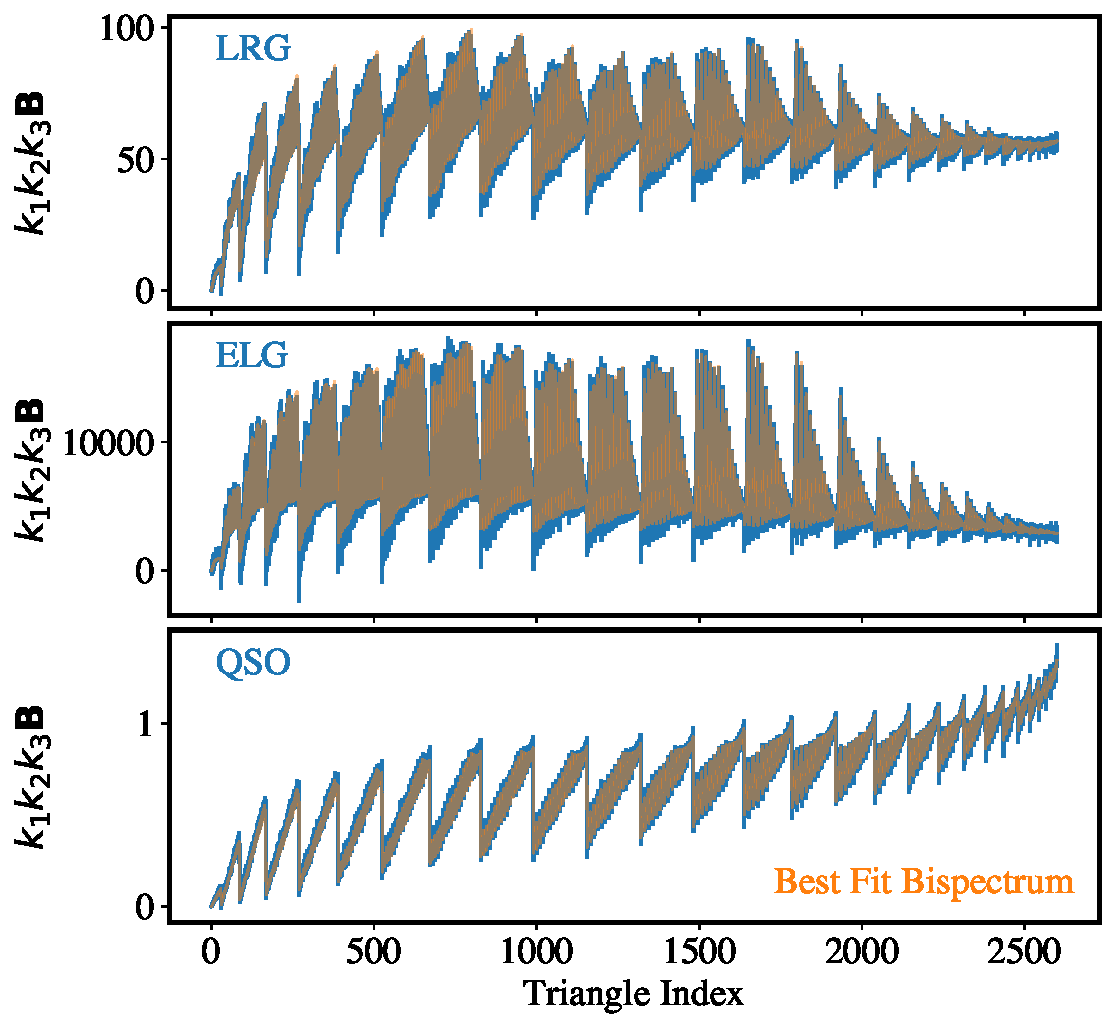
\includegraphics[width=\textwidth]{figures/spectra.pdf}
\caption{Spectra of ABACUS, GLAM, and MOLINO simulations. Top: Mean bispectrum and power spectrum of simulations relative to smooth spectrum either from the mocks (GLAM) or fitting formula (ABACUS). Bottom: Normalized dispersion of bispectrum and power spectrum.}\label{fig:data}
\end{figure*}


We estimate the reduced covariance matrix from a suite of 15000 simulations (MOLINO) and scale it by the variance of power spectrum or bispectrum for the GLAM or ABACUS realizations.

\begin{equation}
	\mathbb{C}_{Y,Y} = (\sigma_{Y} \otimes \sigma_{Y})_{\rm Mock} ~ (\frac{\mathbb{C}_{Y,Y}}{\sigma_{Y} \otimes \sigma_{Y}})_{\rm MOLINO}
\end{equation}
where $\mathbb{C}$



% \begin{enumerate}
% \item sigma (alpha) vs kmax for P(k), B(k), and joint
% \item min $\chi^{2}$ vs alpha for P(k), B(k), and joint
% \end{enumerate}

%DESI is a great experiment. We need higher order statistics to extract more information. Reconstruction techniques can improve the precision, but the amount of information is limited by cosmic variance. Possible ways to improve is to go higher order statistics. 
%
%Cite Lado's paper that if bispectrum used as a standard ruler, a significant improvement is distance scale can be achieved. Much better than the standard reconstruction. Difficult to model the full bispectrum though. In this paper, we would like to do a standard ruler analysis of bispectrum BAO with different DESI-like tracers. 
%
%We find a factor of X improvement, and what happens at different redshifts. Worse for QSO probably, because of high shotnoise and less bispectrum clustering at higher redshifts. 
%
%
%Sec 2. Glam Section
%Plot Glam with and without BAO measurements.
%Describe Molino's covariance and put some justification. 1 Gpc cub.
%Reference Jayashree's paper that the template works well for a range of redshifts. make a plot for sigma alpha vs kmax, with and without nuisance parameters.
%Use CAMB to get the bao constraints for reconstructed power spectrum with GLAM parameters.
%Sec 3. BAO is DESI samples. Analyse Abacus mocks with template from Jayashree. Renormalize Molino's covariance by the ratio of spectra to get covariance for Abacus. Maybe use Glam and Molino to show that spectra ratio scales proportional to dispersion ratio.
%
%Sec 4. BAO detection level. How well we can fit BAO with a smooth function. Mean Glam' with and without BAO as model 1 and 2, and mean Glam with BAO as data. Chi2 vs alpha.



%\begin{equation}
%\log \mathcal{L} = \Delta r^{\dagger} C^{-1} \Delta r,
%\end{equation}
%where $\Delta r = r(\textbf{k}) - r(\alpha \textbf{k})$ with $r$ being defined as the ratio of
